\newpage
\section{Interpretación y Presentación de Resultados}
\subsection{Enunciado}
Deben incluir una sección en la que interpreten los resultados, explicando:
La cantidad de varianza explicada por los componentes seleccionados.
La importancia de los componentes en términos prácticos para la empresa.

\subsection{Varianza Explicada}
Para explicar la varianza, necesitamos ver qué porcentaje cubrimos de la información. Para ello lo reflejaremos en una gráfica:


\begin{figure}[H]
    \centering
    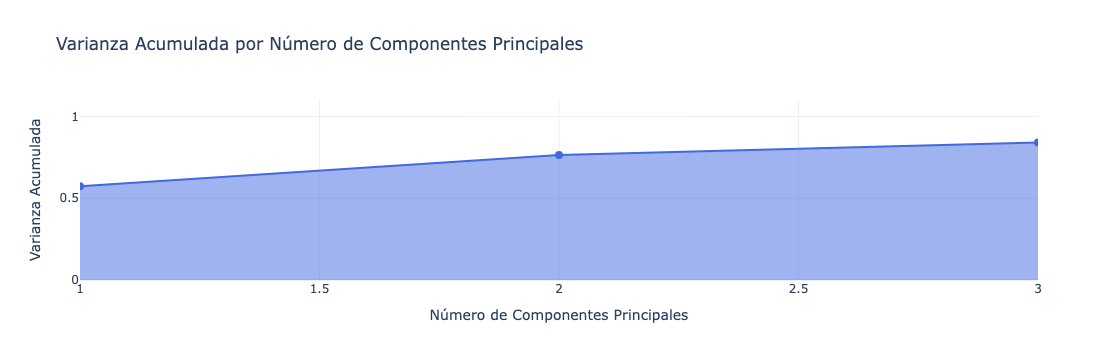
\includegraphics[width=1\textwidth]{images/varianza_acumulada_componentes_principales.png}
    \caption{Varianza Acumulada de los Componentes Principales}
    \label{fig:variance_acum_main_components}
\end{figure}

\begin{table}[h!]
    \centering
    \begin{tabular}{|l|r|}
    \hline
    \textbf{Componentes} & \textbf{Varianza Acumulada} \\ \hline
    PC1                  & 0.57  \\ \hline
    PC2                  & 0.76  \\ \hline
    PC2                  & 0.84  \\ \hline
    \end{tabular}
    \caption{Varianza Acumulada}
\end{table}

Vemos que estamos cubriendo el 84\% de la información.

\subsection{Componentes Principales}

Para explicar los componentes principales y su relación con las variables originales, tenemos que obtener el \textbf{Loading Vector} \\

Este gráfico refleja la relación a un nivel general, pero es importante porque te brinda un panorama rápido de relación. Con una
primera observación podríamos decir que el PC1 está bastante distribuída y son positivas todas sus variables.

\begin{figure}[H]
    \centering
    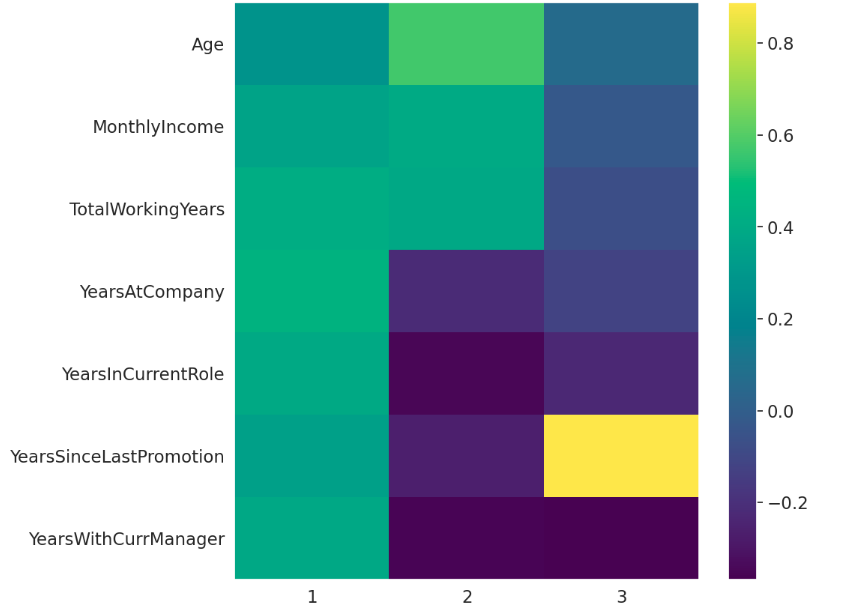
\includegraphics[width=1\textwidth]{images/heatmap_main_component.png}
    \caption{Mapa de Calor de Componentes Principales vs Variables Originales}
    \label{fig:heatmap_main_component}
\end{figure}

\subsubsection{PC1}

Este componente describe la Experiencia Laboral desde el punto de vista de años.
En términos de importancia para la empresa, refleja que se tiene personal con bastante experiencia laboral
y que no tienen una edad avanzada, lo cuál refleja que hay relación entre la edad y la experiencia pero en la empresa
no lo tienen tan pronunciado.

\begin{figure}[H]
    \centering
    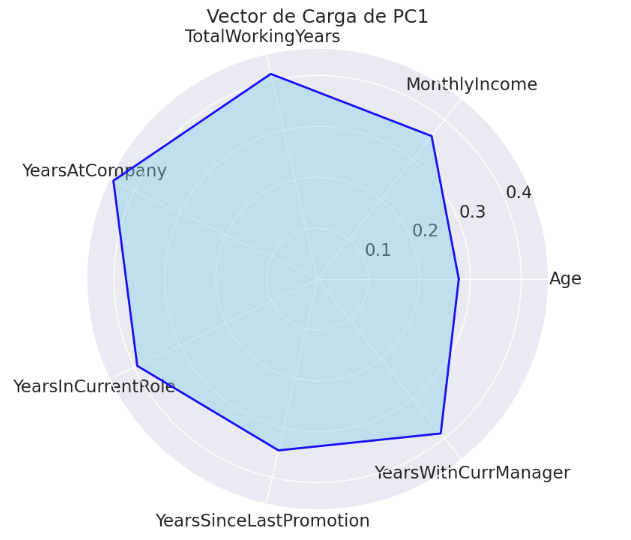
\includegraphics[width=1\textwidth]{images/pollar_pc1.png}
    \caption{Vector de Carga PC1}
    \label{fig:vector_pc1}
\end{figure}

\subsubsection{PC2}

Podemos describir como un componente que describe una fuerta Experiencia Laboral no necesariamente en la compañía y su Edad
Pero también muestra que esa experiencia laboral en cuanto a tiempo no lo tiene en la empresa y en especial tiene
poco tiempo con un manager.

\begin{figure}[H]
    \centering
    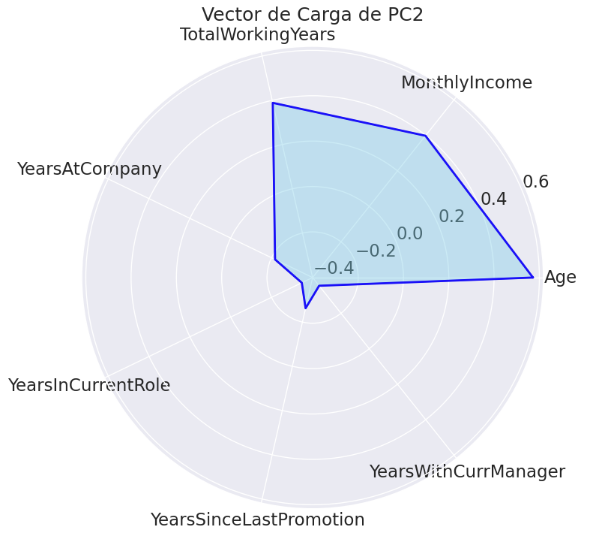
\includegraphics[width=1\textwidth]{images/pollar_pc2.png}
    \caption{Vector de Carga PC2}
    \label{fig:vector_pc2}
\end{figure}

\subsubsection{PC3}

Este componente muestra que existen empleados en la empresa que desde hace mucho tiempo
no han sido promovidos, muy posible por un factor de tiempo en la compañía.

\begin{figure}[H]
    \centering
    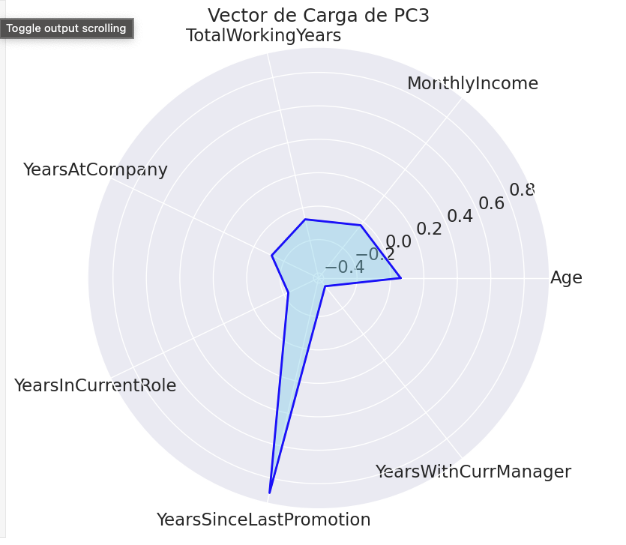
\includegraphics[width=1\textwidth]{images/pollar_pc3.png}
    \caption{Vector de Carga PC3}
    \label{fig:vector_pc3}
\end{figure}

